\section{Durchführung}
Der Aufbau ist in Abbildung (\ref{abb:1}) dargestellt.
\begin{figure}[H]
  \centering
  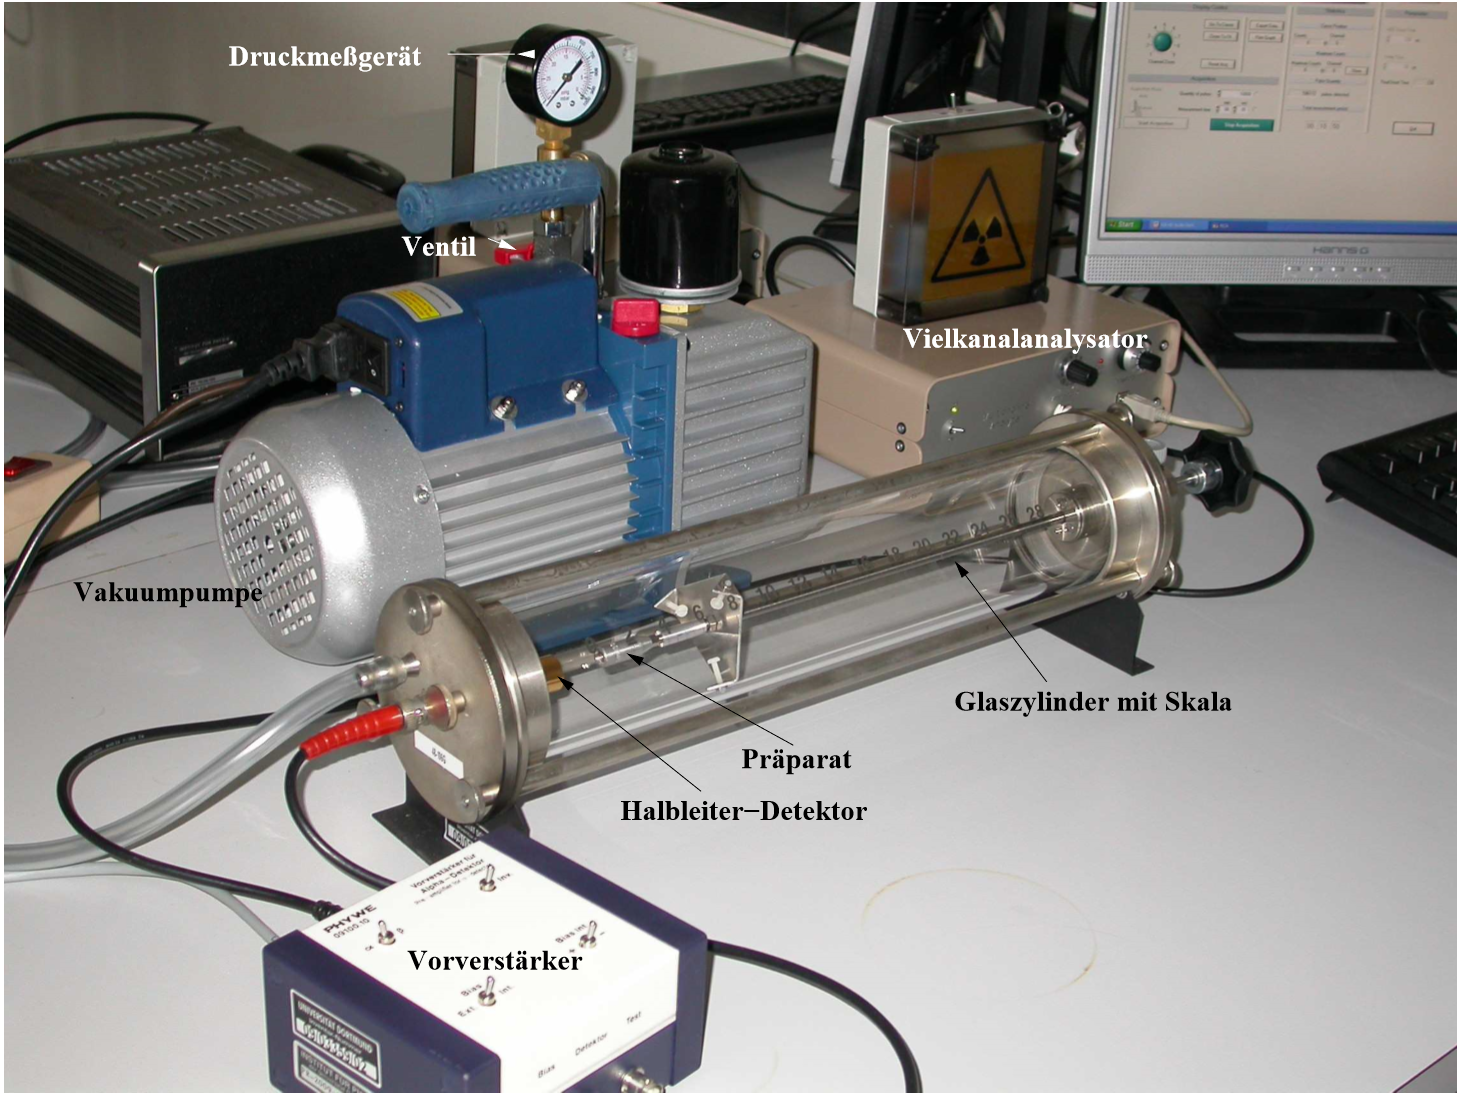
\includegraphics[width=\textwidth]{content/Aufbau.png}
  \caption{Experimenteller Aufbau zur Bestimmung der $\alpha$-Strahlung \cite{1}.}
  \label{abb:1}
\end{figure}
Als Strahlungquelle für $\alpha$-Teilchen wird ein Am-Präparat verwendet.
Der Strahler befindet sich auf einem verschiebbaren Halter, sodass der Abstand $x$
zwischen $\alpha$-Präparat und Detektor variiert werden kann. Als Detektor
wird ein Halbleiter-Sperrschichtzähler verwendet. Fällt ein Ion in die Verarmungszone
ein, enstehen Elektronen-Loch Paare die zu einem Strompuls führen. Dieser Puls wird
vom Vorverstärker verstärkt und in einem Vielkanalanalysator nach seiner Pulshöhe analysiert. Wichtig hierbei
ist das die Energie des Teilchens $\propto $ zur Pulshöhe ist.
Das in Abbildung (\ref{abb:1}) verwendete Druckmessgerät dient zur Evakuierung des Glaszylinders.
Zur Aufnahme dient ein Rechner, der zum einen die Gesamtzählrate als auch die Energie anzeigt.
